\documentclass[12pt]{report}

\usepackage[norsk]{babel}
\usepackage{graphicx, array, carlito, fancyhdr, comment, etoc, lipsum, enumitem, standalone, subfiles, newclude, float, enumitem, amsmath, adjustbox, titlesec, pdfpages}

% TIDLIGERE BIB Basert på biblatex eller noe...
\usepackage[style=ieee, sorting=none]{biblatex}
\addbibresource{backmatter/referanser.bib}


\usepackage[hidelinks]{hyperref}
% Fjerne Teksten Kapittel fra overskrift. Justerer plasseringen av chapter navn
\titleformat{\chapter}[display]
{\Huge\bfseries}
{}
{-120pt}
{\thechapter.\ }
\titleformat{name=\chapter,numberless}[display]
{\Huge\bfseries}
{}
{-120pt}
{}
\titlespacing*{\chapter}{0pt}{70pt}{10pt} % Juster verdien 40pt for å endre avstanden


%Gir automatisk nytt avsnitt ved linjeskift
\usepackage[parfill]{parskip}

%Ikke inrykk ved nytt avsnitt
\setlength{\parindent}{0pt}

\usepackage{exsheets}
%Vis løsningsforslag på alle oppgaver
\SetupExSheets{solution/print=false}


\usepackage[a4paper, total={6in, 8in}]{geometry}





% Adding abstract funciton
\newcommand{\chapabstract}[1]{
	\begin{quote}
		\singlespacing\small
		\rule{14cm}{1pt}
		#1
		\vskip-4mm
		\rule{14cm}{1pt}
\end{quote}}


% Set up the fancyhdr package
\pagestyle{fancy}
\fancyhf{} % Clear all header and footer fields

% Adjust the footer position
\setlength{\footskip}{3cm} % You can adjust this value as needed

% Define the footer
%\fancyfoot[L]{\vspace{1cm} \makebox[0pt][l]{\hspace{0.5cm} Elektroniske systemer}} % Left-aligned course name, lifted up
\fancyfoot[R]{%
	\begin{minipage}{2cm}
		\centering
		
\includegraphics[height=1cm]{frontmatter/bilder/r171JViZ6gmf8WXujFQw.jpg}\\
%		\vspace{-0.5cm} % Adjust vertical space to center page number
%		\thepage
	\end{minipage}
}
%\fancyfoot[C]{\thepage}

\fancyhead{}
\fancyhead[LE,RO]{\nouppercase{\rightmark}}
\fancyhead[RE,LO]{Side \thepage}





% ------------------    HER STARTER DOKUMENTET   ------------------

\begin{document}
%Setter inn tittelsiden som eksternt dokument
\begin{titlepage}
    \begin{center}
    \vspace*{1cm}
    \Huge
    \textbf{Elektroniske systemer}
    
    \LARGE
    \vspace{0.5cm}
    Øvingsoppgaver for analoge komponenter og måleteknikk i emnet elektroniske systemer

    \vspace{1.5cm}
    \textbf{Carl Magnus Bøe}
    
    2025

\vfill




    
\includegraphics[width=0.6\textwidth]{frontmatter/bilder/r171JViZ6gmf8WXujFQw.jpg}
    \Large
    
    Fagskolen Viken\\
    01TE00F EITKELFH24\\
    Fredrikstad\\

    \end{center}
\end{titlepage}

%Innholdsfortegnelse
\tableofcontents
\chapter{Introduksjon}
\label{ch:introduksjon}
Dette kapittelet inneholder generell informasjon om kompendiet med bakgrunn for arbeidet, oppbygging av dokumentet og lisensinformasjon.

\section{Bakgrunnsinformasjon}
Dette dokumentet er et kompendium som inneholder øvingsoppgaver relevante for delen analoge komponenter i emnet elektroniske systemer. Siden dokumentet blir kontinuerlig revidert, er det datomerkingen på forsiden som angir versjonen av dokumentet. Målet med dette dokumentet er å samle alle øvingsoppgaver sammen med løsningsforslagene i ett dokument.

Når man jobber med oppgavene, anbefales det at man også gjør simuleringer. %Noen anbefalte simuleringsverktøy er omtalt i Kapittel \ref{ch:programvare}.

Dersom du har kommentarer, forslag til oppgaver eller har funnet noe som er feil, vennligst send en epost til \href{mailto:carlbo@afk.no}{carlbo@afk.no}.

\section{Oppbygning av kompendiet}
Kompendiet er delt opp i hovedgrupper, hvor undergrupper som forskjellige elektroniske komponenter er beskrevet som seksjoner. For hver seksjon presenteres først alle oppgavene, før løsningsforslaget blir presentert i neste seksjon.

\begin{comment}
	\section{Lisensinformasjon}
	Dette dokumentet er basert på materiale fra \textit{Lessons In Electric Circuits} av Tony R. Kuphaldt, distribuert under Design Science License. Originaldokumentet kan finnes på \href{https://www.ibiblio.org/kuphaldt/electricCircuits/}{Lessons In Electric Circuits}. Eventuelle modifikasjoner og avledede verk er også distribuert under Design Science License.
	
	Deler av dette kompendiet er utviklet av Carl Magnus Bøe. Disse delene inkluderer:
	\begin{enumerate}[label=\roman*)]
		\item Kapittel \ref{sec:diodeOppgave} / \ref{sec:diodeLøsning}
		\item 
	\end{enumerate}
\end{comment}
%\chapter{Programvare}
\label{ch:programvare}
Dette kapittelet omtaler forskjellig programvare relevant i emnet.


\section{Simulering}
\subsection{CircuitMaker2000}
\href{https://winworldpc.com/product/circuitmaker/2000}{CircuitMaker2000}
\subsection{LTspice}
\href{https://www.analog.com/en/resources/design-tools-and-calculators/ltspice-simulator.html}{LTspice}
\subsection{OpenModelica}
\href{https://openmodelica.org/}{OpenModelica}

\section{Tegne kretser}
\subsection{Draw.io}


\chapter{Analoge komponenter}

\section{Dioder}


Dette kapittelet inneholder oppgaver relatert til halvleder dioder. Om ingenting annet er gitt i oppgaven så antar vi et ideelt spenningsfall over dioden på $0,7[V]$.\\
\subsection{Lysdioder - LED}
Lysdioder har forskjellige spenningsfall for samme farge avhengig av modellserie og produsent. For optimal verdi må man lese databladet til dioden. 

Tabell \ref{tab:LEDspenningsfall} viser et generelt spenn av verdier.

\begin{table}[!ht]
	\caption{Spenningsfall for forskjellige lysdioder}
	\label{tab:LEDspenningsfall}
	\begin{center}
		\begin{tabular}{|l|c|c|} 
			\hline
			Farge & Spenningsfall & Enhet \\ [0.5ex] 
			\hline\hline
			Hvit & $3,0 - 5,0$ &$ [V]$ \\
			\hline
			Fiolett: &  $2,8 - 4,0$ &$ [V]$\\
			\hline
			Blå: &  $2,5 - 3,7$ &$ [V]$\\
			\hline
			Grønn: &  $1,6 - 4,0$ &$ [V]$\\
			\hline
			Gul: &  $2,0 - 2,4$ &$ [V]$\\
			\hline
			Oransje: &  $2,0 - 2,1$ &$ [V]$\\
			\hline
			Rød: &  $1,5 - 2,0$ &$ [V]$\\
			\hline
			Infrarød: &  $1,2 - 1,9$ &$ [V]$\\
			\hline
		\end{tabular}
	\end{center}
\end{table}



%Setter inn oppgaver fra ekstern ark
\subsection{Oppgaver}
\label{sec:diodeOppgave}
\subsubsection{Dioder}
\input{diode/oppgaver_dioder}
\subsubsection{Zenerdioder}
\input{diode/oppgaver_zenerdioder}
\subsection{Løsningsforslag}
\label{sec:diodeLøsning}
\printsolutions[section]

\newpage

\section{Tyristor, triac og diac}
%Dette er tyristorarket

\subsection{Oppgaver}
\begin{question}[name=Spørsmål, topic=tyristor]
	Tegn symbolene for følgende komponenter.
	\begin{enumerate}[label=\roman*]
		\item Halvlederdiode
		\item LED
		\item Zenerdiode
	\end{enumerate}
\end{question}


\begin{solution}[name=Løsningsforslag]
tatata

%	\begin{figure}[H]
%		\centering
%		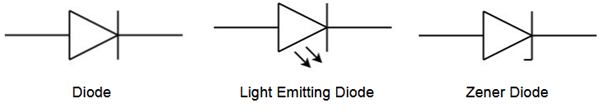
\includegraphics[width=0.7\textwidth]{diode/figurer/oppgave1.png}
%		\caption{Eksempel på forskjellige diode symboler.}
%		\label{fig:diodeSeeeymb}
%	\end{figure}
\end{solution}
\subsection{Løsningsforslag}
\printsolutions[section]

\newpage

\section{Transistor - BJT}
\label{sec:tranBJT}

\subsection{Oppgaver}
%\SetupExSheets{headings=block}

% ------------------ MALER ------------------
\begin{comment}

\begin{question}[name=Oppgave, topic=transBJT]

	\begin{enumerate}[label=\roman*)]

	\end{enumerate}
\end{question}

\vspace{0.5cm} % Add space after the solution

\begin{solution}[name=Løsningsforslag oppgave]

	\begin{figure}[H]
		\centering
		\includegraphics[width=0.7\textwidth]{}
		\caption{}
		\label{fig:}
	\end{figure}
\end{solution}

\vspace{0.5cm} % Add space after the solution
\end{comment}

\begin{question}[name=Oppgave, topic=transBJT]
	\begin{enumerate}[label=\roman*)]
		\item Hva heter de tre tre forskjellig strømmene i en BJT-transistor?
		\item Hvilken av strømmene i en BJT-transistor er vanligvis den største?
		\item Hva er forskjellen mellom saturation og cut-off for en transistor?
		\item Hva beskriver strømforsterkningen $B$?
	\end{enumerate}

\end{question}

\vspace{0.5cm} % Add space after the solution

\begin{solution}[name=Løsningsforslag oppgave]
		\begin{enumerate}[label=\roman*)]
		\item Kollektor-strøm, emitter-strøm og basis-strøm
		\item Emitter er vanligvis den største siden den er summen av kollektor og basestrømmen
		\item Saturation oppstår når transistoren leder maksimalt og spenningsfallet mellom kollektor og emitter er $\approx 0 [V]$.
		
		Cut-off oppstår når det ikke går noen kollektor-strøm og nesten hele det maksimale spenningsfallet ligger over transistorens kollektor og emitter pinner.
		\item Forholdet mellom kollektor-strømmen og base-strømmen.
	\end{enumerate}

\end{solution}

\vspace{0.5cm} % Add space after the solution


\begin{question}[name=Oppgave, topic=transBJT]
Basert på kretsen presentert i Figur \ref{fig:tranBJT1} Beregn verdiene for $I_B$, $I_C$, $I_E$ og $U_{CE}$. Anta en strømforsterkning $\beta =75$ og spenningsfall $U_{BE}=0,7[V]$.

	\begin{figure}[H]
		\centering
		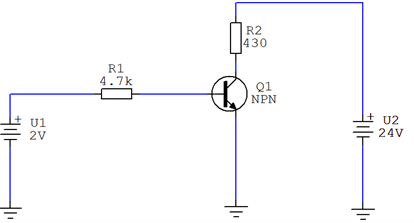
\includegraphics[width=0.7\textwidth]{transistor-BJT/figurer/krets1.png}
		\caption{Krets med BJT-transistor}
		\label{fig:tranBJT1}
	\end{figure}

\end{question}

\vspace{0.5cm} % Add space after the solution

\begin{solution}[name=Løsningsforslag oppgave]
Finner først basis-strømmen.
\[I_B=\frac{U_1-U_{BE}}{R_1}=\frac{2-0,7}{4,7\cdot 10^3}\approx 0,277 [mA]\]

Bruker strømforsterkningen $ \beta $ for å finne strømmen $I_K$.
\[\beta=\frac{I_C}{I_B} \rightarrow I_C= \beta \cdot I_B=75\cdot0,277 \cdot10^{-3} \approx 20,7[mA]\]


Finner så strømmen  $I_C$.
\[I_B+I_C+I_E=0 \rightarrow I_C=I_E-I_B=20,7\cdot 10^{-3} - 0,277 \cdot 10^{-3} \approx 20,42 [mA]\]

Beregner spenningsfallet $U_{BE}$.
\[U_{CE}=U_2-U_{R2}=U_2-(R_2 \cdot I_C) =24-(430 \cdot 20,42 \cdot 10^{-3}) \approx 15,2[V]\]
	
\end{solution}

\vspace{0.5cm} % Add space after the solution

\begin{question}[name=Oppgave, topic=transBJT]
	Basert på kretsen presentert i Figur \ref{fig:tranBJT2} Beregn verdiene for $I_B$, $I_C$, $I_E$ og $U_{CE}$. Anta en strømforsterkning $\beta=250$ og spenningsfall $U_{BE}=0,7[V]$.
	
	\begin{figure}[H]
		\centering
		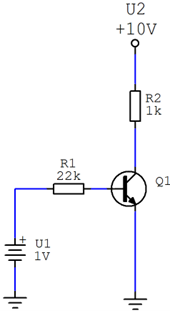
\includegraphics[width=0.25\textwidth]{transistor-BJT/figurer/krets2.png}
		\caption{Krets med BJT-transistor}
		\label{fig:tranBJT2}
	\end{figure}
	
\end{question}

\vspace{0.5cm} % Add space after the solution

\begin{solution}[name=Løsningsforslag oppgave]
Finner basis-strømmen.
\[I_B=\frac{U_{R1}}{R_1}= \frac{1-0,7}{22 \cdot 10^3} \approx 13,64 [\mu A]\]
Bruker transistorens formel for strømforsterkning til å finne emitter-strømmen.
\[I_E=\beta \cdot I_B =250 \cdot 13,64 \cdot 10^{-6} \approx 3,41 [mA]\]

Den relativt store forsterkningen gjør at antall desimaler brukt i $I_B$ vil påvirke nøyaktigheten på $I_E$ i stor grad.

I dette tilfellet er $I_K >>\footnote{Tegnet betyr mye større enn. Eksempel: $9\cdot10^{9}>>1\cdot10^{-10}$} I_B$ og vi kan derfor forenkle beregningen ved å anta $I_E = I_K$

\[U_{CE} = U_2-U_{R_{2}}=10-(1\cdot 10^3 \cdot 3,41 \cdot 10^{-3}) = 6,59 [V] \]


\end{solution}
\vspace{0.5cm} % Add space after the solution
\begin{question}[name=Oppgave, topic=transBJT]
	Basert på kretsen presentert i Figur \ref{fig:tranBJT3} Beregn verdiene for $I_C$, $I_E$, $U_B$ og $U_{BE}$. Anta spenningsfall $U_{BE}=0,7[V]$.
	
	\begin{figure}[H]
		\centering
		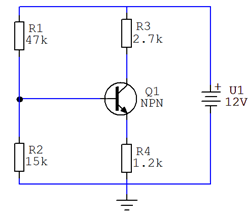
\includegraphics[width=0.45\textwidth]{transistor-BJT/figurer/krets3.png}
		\caption{Krets med BJT-transistor}
		\label{fig:tranBJT3}
	\end{figure}
	
\end{question}

\vspace{0.5cm} % Add space after the solution

\begin{solution}[name=Løsningsforslag oppgave]
Finner spenninging $U_B$

\[U_B= \left(\frac{R_2}{R_1+R_2} \right) \cdot U_1 = \left(\frac{15 \cdot 10^3}{47 \cdot 10^3 + 15 \cdot 10^3} \right) \cdot 12 = 2,9 [V]\]

Beregner emitterspenningen basert på spenningsfallene  $U_B$ og $U_{BE}$.
\[U_E = U_B - U_{BE}=2,90-0,7=2,2 [V]\]

\[I_E = \frac{U_4}{R_4}=\frac{2,2}{1,2 \cdot 10^3} \approx 1,833 [mA]\]

Antar $I_C = I_E$.

Finner totale spenningsfallet fra kollektor-pinnen til jord. Dette er summen av to spenningsfall $U_{CE}$ og $U_{R_{4}}$.
\[U_C = U_1-U_{R_{3}}=U_1-(I_C \cdot R_3)=12-(1,833 \cdot 10^{-3} \cdot 2,7 \cdot 10^{3})=7,1 [V]\]

Trekker fra spenningsfallet over $U_{R_{4}}$ fra $U_C$ for å finne spenningsfallet over transistoren $U_{CE}$.

\[U_{KE} = U_K-U_E=7,1-2,2=4,9 [V]\]

\end{solution}

\vspace{0.5cm} % Add space after the solution


\begin{question}[name=Oppgave, topic=transBJT]
	Basert på kretsen presentert i Figur \ref{fig:tranBJT4} Beregn verdiene for $I_B$, $I_C$, $I_E$ og $U_C$. Anta spenningsfall $U_{BE}=0,7[V]$ og $\beta=90$.
	
	\begin{figure}[H]
		\centering
		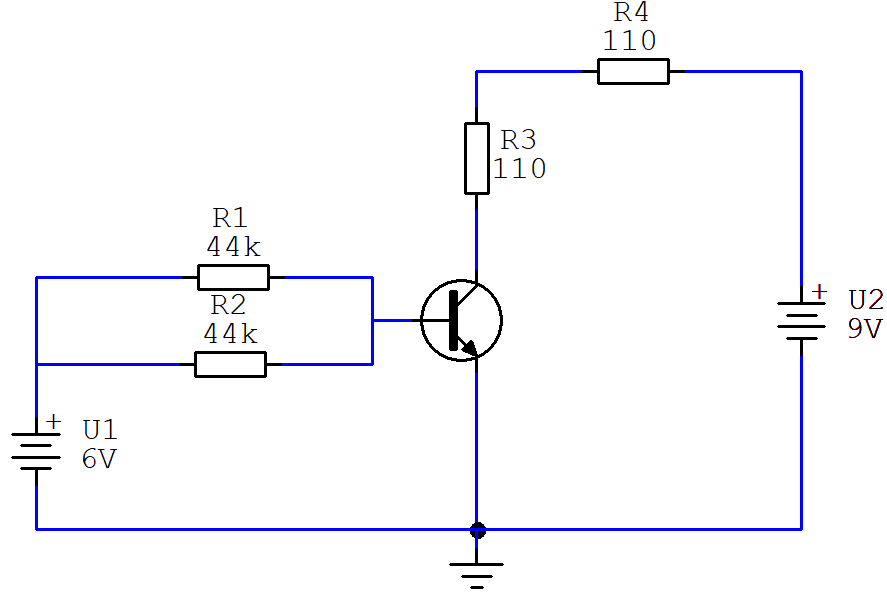
\includegraphics[width=0.6\textwidth]{transistor-BJT/figurer/krets4.png}
		\caption{Krets med BJT-transistor}
		\label{fig:tranBJT4}
	\end{figure}
	
\end{question}

\vspace{0.5cm} % Add space after the solution

\begin{solution}[name=Løsningsforslag oppgave]
Beregner resistansen for basis-strømmen.

\[R_B= \left(\frac{1}{R_1} + \frac{1}{R_2} \right)^{-1} = \left( \frac{1}{44\cdot 10^3} + \frac{1}{44 \cdot 10^3}\right)^{-1}= 22 [k\Omega]\]

Finner $I_B$.

\[I_B = \frac{U_1-U_{BE}}{R_B} = \frac{9-0,7}{22 \cdot 10^3} \approx 0,377 [mA]\]

Bruker forsterkningen $\beta$ til å finne $I_E$.

\[I_E = \beta \cdot I_B = 90 \cdot 0,377 \cdot 10^{-3} \approx 34 [mA] \]

\[I_C = I_C - I_B = 34 \cdot 10^{-3} - 0,377 \cdot 10^{-3} = 33,623 [mA]\]

Finner spenningen $U_C$ som er spenningsfallet mellom kollektor-pinnen og jord.

Summerer kollektor-motstandene
\[R_K = R_3+R_4=110+110=220 [\Omega]\]

\[U_C=U_2-U_{R_{K}} = U_2 - \left( R_K \cdot I_K \right)=9- \left( 220 \cdot 33,623 \cdot 10^{-3} \right) \approx 7,4 [V]\]

\end{solution}

\vspace{0.5cm} % Add space after the solution

\begin{question}[name=Oppgave, topic=transBJT]
	Basert på kretsen presentert i Figur \ref{fig:tranBJT5} Finn motstandsverdien for $R_1$ slik at strømmen i $I_C=120 [mA]$. Anta spenningsfall $U_{BE}=0,7[V]$ og $\beta=96$.
	
	\begin{figure}[H]
		\centering
		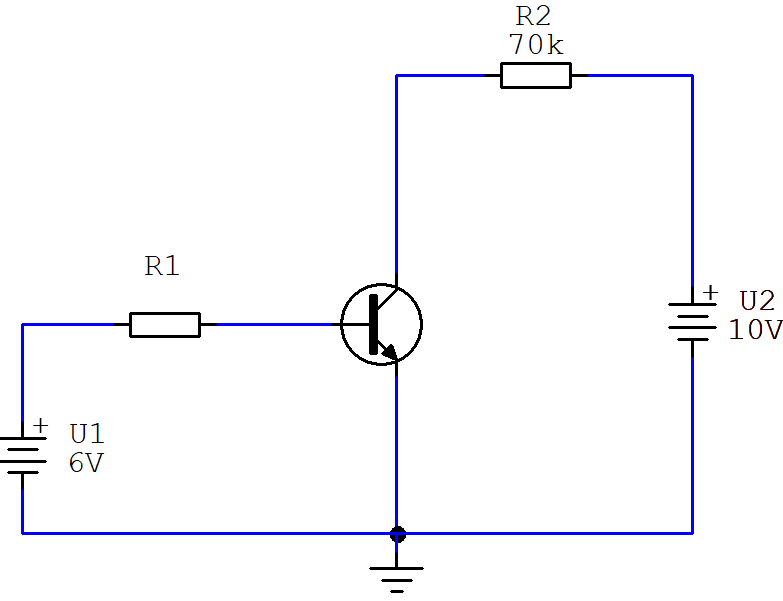
\includegraphics[width=0.6\textwidth]{transistor-BJT/figurer/krets5.png}
		\caption{Krets med BJT-transistor}
		\label{fig:tranBJT5}
	\end{figure}
	
\end{question}

\vspace{0.5cm} % Add space after the solution

\begin{solution}[name=Løsningsforslag oppgave]
\[\beta = \frac{I_C}{I_B} \rightarrow I_B = \frac{I_C}{\beta} \rightarrow I_B= \frac{120 \cdot 10^{-3}}{96} = 1,25[mA]\]

\[R_1= \frac{U_{R_{1}}}{I_B} = \frac{6-0,7}{1,25 \cdot 10^{-3}}=4,24[k\Omega] \]

\end{solution}

\vspace{0.5cm} % Add space after the solution

\begin{question}[name=Oppgave, topic=transBJT]
	
Finn motstandsverdiet for $R_B$ og $R_K$ for kretsen presentert i Figur \ref{fig:tranBJT6}.
	
Kretsen skal dimensjoneres til å ha følgende verdier:
\[U_{KE}=6[V]\]
\[U_{BE}=0,7[V]\]
\[I_K=6[mA]\]

Transistoren $Q_1$ har oppgitt $ \beta= 150$ og spenningen for kilden $ U_b=12[V]$
	
	\begin{figure}[H]
		\centering
		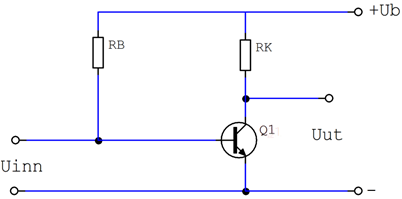
\includegraphics[width=0.6\textwidth]{transistor-BJT/figurer/krets6.png}
		\caption{Krets med BJT-transistor}
		\label{fig:tranBJT6}
	\end{figure}
	
\end{question}

\vspace{0.5cm} % Add space after the solution

\begin{solution}[name=Løsningsforslag oppgave]
\[\beta = \frac{I_C}{I_B} \rightarrow I_B=\frac{I_K}{\beta}=\frac{6 \cdot 10^{-3}}{150} = 40[\mu A]\]

\[R_B=\frac{U_B-U_{BE}}{I_B}= \frac{12-0,7}{40 \cdot 10^{-6}}=282,5[k\Omega] \]

\[R_K=\frac{U_B-U_{KE}}{I_K}= \frac{12-6}{6 \cdot 10^{-3}}=1[k\Omega]\]

\end{solution}


\begin{question}[name=Oppgave, topic=transBJT]
Ta utgangspunkt å Figur \ref{fig:tranBJT7}. Det er brudd i $R_1$. Hva blir verdien for $U_B$, $U_E$ og $U_C$?

	\begin{figure}[H]
		\centering
		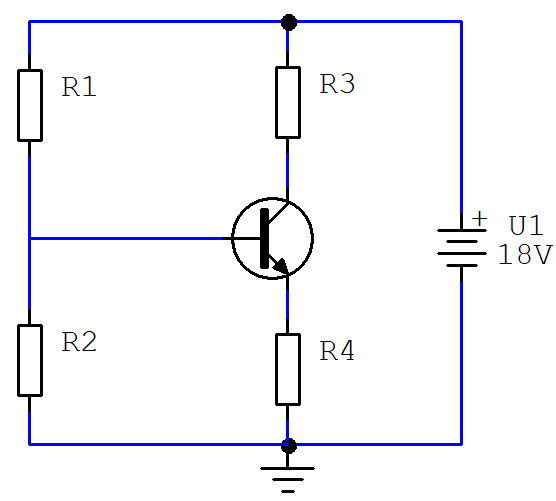
\includegraphics[width=0.5\textwidth]{transistor-BJT/figurer/krets7.png}
		\caption{Krets med BJT-transistor}
		\label{fig:tranBJT7}
	\end{figure}
	
\end{question}

\vspace{0.5cm} % Add space after the solution

\begin{solution}[name=Løsningsforslag oppgave]
	$U_B=0[V]$, $U_E=0[V]$ og $U_C=18[V]$
	Her vil transistoren være i cut-off. Det vil ikke gå noen strøm $I_B$ og transistoren vil derfor ikke lede. Hele spenningen til kilden vil ligge over $U_C$.

\end{solution}




\begin{question}[name=Oppgave, topic=transBJT]
Ta utgangspunkt i kretsen som vist i Figur \ref{fig:tranBJT8} og beregn $I_C$, $U_1$, $\beta$ og $R_1$
	
	\begin{figure}[H]
		\centering
		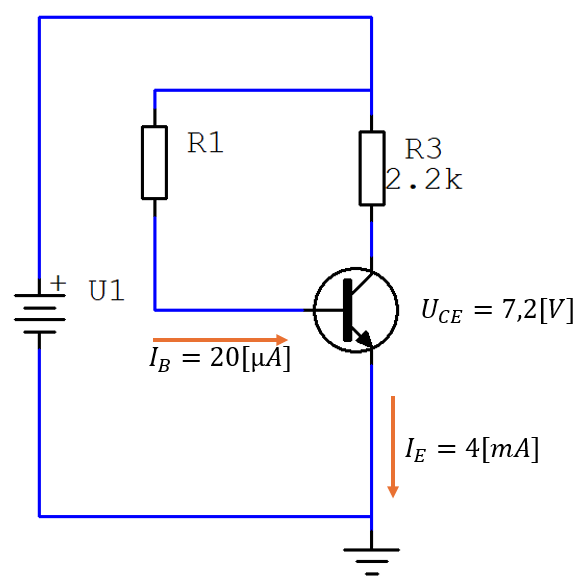
\includegraphics[width=0.5\textwidth]{transistor-BJT/figurer/krets8.png}
		\caption{Krets med BJT-transistor}
		\label{fig:tranBJT8}
	\end{figure}
	
\end{question}

\vspace{0.5cm} % Add space after the solution

\begin{solution}[name=Løsningsforslag oppgave]
\[I_C=I_E - I_C=4 \cdot 10^{-3} - 20 \cdot 10^{-6}= 3,98[mA]\]

\[U_1 = U_{R_C}+U_{CE} = (I_C \cdot R_C)+U_{CE}=(3,98 \cdot 10^{-3} \cdot 2,2 \cdot10^3) + 7,2 = 15,96 [V]\]

\[\beta=\frac{I_C}{I_B}=\frac{3,98 \cdot 10^{-3}}{20 \cdot 10^{-6}}=199\]

\[R_B=\frac{U_B}{I_B}= \frac{15,96-0,7}{20 \cdot 10^{-6}}=763 [k\Omega]\]


\end{solution}
\subsection{Løsningsforslag}
\printsolutions[section]

\newpage



%\section{FET transistor}

\section{Forsterkning}
\label{sec:forsterk}

\subsection{Oppgaver}
\SetupExSheets{headings=block}
\subsection{Løsningsforslag}
\printsolutions[section]

\newpage

\section{Operasjonsforsterker}
\label{sec:opamp}

\subsection{Oppgaver}
% Templates
\begin{comment}

\begin{figure}[H]
	\centering
	\includegraphics[width=0.7\textwidth]{operasjonsforsterker/}
	\caption{}
	\label{fig:}
\end{figure}

\vspace{0.5cm} % Add space after the solution

\begin{enumerate}[label=\roman*)]
	\item
	\item
\end{enumerate}

\begin{question}[name=Oppgave, topic=operasjonsforsterker]

	\begin{enumerate}[label=\roman*)]
		\item
		\item
		\item
	\end{enumerate}
\end{question}

\vspace{0.5cm} % Add space after the solution

\begin{solution}[name=Løsningsforslag oppgave]
	Symboler vist i Figur \ref{fig:}.
	\begin{figure}[H]
		\centering
		\includegraphics[width=0.7\textwidth]{}
		\caption{}
		\label{fig:}
	\end{figure}
\end{solution}
\end{comment}

%--------------------------- GENERELT --------------------------------
\begin{question}[name=Oppgave, topic=operasjonsforsterker]
	En integrert operasjonsforsterker har
	\begin{enumerate}[label=\roman*)]
		\item To innganger og to utganger
		\item Én inngang og én utgang
		\item To innganger og én utganga
	\end{enumerate}
\end{question}

\begin{solution}[name=Løsningsforslag oppgave]
	Riktig svar: iii

\end{solution}
\vspace{0.5cm} % Add space after the solution
\begin{question}[name=Oppgave, topic=operasjonsforsterker]
	Hvilken av disse egenskapene beskriver en operasjonsforsterker dårligst
	\begin{enumerate}[label=\roman*)]
		\item Høy forsterkning
		\item Høy inngangsmotstand
		\item Lav effekt
		\item Lav utgangsresistans
	\end{enumerate}
\end{question}

\begin{solution}[name=Løsningsforslag oppgave]
	Riktig svar: iii

\end{solution}
\vspace{0.5cm} % Add space after the solution
\begin{question}[name=Oppgave, topic=operasjonsforsterker]
	Med $0[V]$ på begge inngangene skal en ideell operasjonsforsterker ha hva på utgangen
	\begin{enumerate}[label=\roman*)]
		\item Positiv driftspenning $+V_{cc}$
		\item Negativ driftspenning $-V_{cc}$
		\item $0[V]$
	\end{enumerate}
\end{question}

\begin{solution}[name=Løsningsforslag oppgave]
	Riktig svar: iii

\end{solution}
\vspace{0.5cm} % Add space after the solution
\begin{question}[name=Oppgave, topic=operasjonsforsterker]
	Av verdiene nevnt i listen, hvilken at de beskriver den mest realistiske verdien for operasjonforsterkerens forsterkning uten tilbakekobling.
	\begin{enumerate}[label=\roman*)]
		\item 1
		\item 2000
		\item 80[dB]
		\item 100000
	\end{enumerate}
\end{question}

\begin{solution}[name=Løsningsforslag oppgave]
	Riktig svar: iv
\end{solution}
\vspace{0.5cm} % Add space after the solution

\begin{question}[name=Oppgave, topic=operasjonsforsterker]
	Velg det riktige alternativet for egenskapene til en ideell operasjonsforsterker.

	\begin{enumerate}[label=\roman*)]
		\item Hvilke tilkoblinger har en standard operasjonsforsterker?
		\item Hvordan er spenningsforsterkning for en ideell operasjonsforsterker annerledes enn for en fysisk operasjonsforsterker?
		\item Hva indikerer $+$ tegnet på den ene inngangen av operasjonsforsterkeren?
		\item
	\end{enumerate}
\end{question}

\vspace{0.5cm} % Add space after the solution

\begin{solution}[name=Løsningsforslag oppgave]

	\begin{enumerate}[label=\roman*)]
		\item Inverterende og ikke-inverterende innganger, utgang, positiv og negativ tilførsel
		\item En fysisk operasjons-forsterker har stor spenningsforsterkning, men ikke uendelig som vi antar for den ideelle modellen
		\item Ikke-inverterende inngang
	\end{enumerate}

\end{solution}

\vspace{0.5cm} % Add space after the solution
\begin{question}[name=Oppgave, topic=operasjonsforsterker]
Velg det riktige alternativet for egenskapene til en ideell operasjonsforsterker.

	\begin{enumerate}[label=\roman*)]
	\item Inngangsimpedans = 0 og utgangsimpedans = 0
	\item Inngangsimpedans = 0 og utgangsimpedans = $\infty$
	\item Inngangsimpedans = $\infty$ og utgangsimpedans = 0
	\item Inngangsimpedans = $\infty$ og utgangsimpedans = $\infty$
\end{enumerate}
\end{question}

\vspace{0.5cm} % Add space after the solution

\begin{solution}[name=Løsningsforslag oppgave]
	Riktig svar er iii.

\end{solution}
\vspace{0.5cm} % Add space after the solution


\begin{question}[name=Oppgave, topic=operasjonsforsterker]
Ta utgangspunkt i delenummer TL081P og det vedlagte databladet presentert i Vedlegg \ref{paper-b} for å svare på følgende:
	\begin{enumerate}[label=\roman*)]
	\item Tegn opp en prinsippskisse for hvordan man kan koble opp en inverterende og ikke-inverterende kobling
	\item Hva er den maksimale spenningen brikken kan drives med, og hva er den maksimale spenningen den bør drives med.
	\item Hva er den maksimale spenningen man kan ha inn på inngangen
	\end{enumerate}



\end{question}

\vspace{0.5cm} % Add space after the solution

\begin{solution}[name=Løsningsforslag oppgave]


\end{solution}
\vspace{0.5cm} % Add space after the solution


\begin{question}[name=Oppgave, topic=operasjonsforsterker]
Studer kretsene vist i Figur \ref{fig:basicOpamp1}, Figur \ref{fig:basicOpamp2} og Figur \ref{fig:basicOpamp3} forså å angi hva utgangspenningen er for de forskjellige koblingene.

	\begin{figure}[H]
		\centering
		\begin{minipage}{0.45\textwidth}
			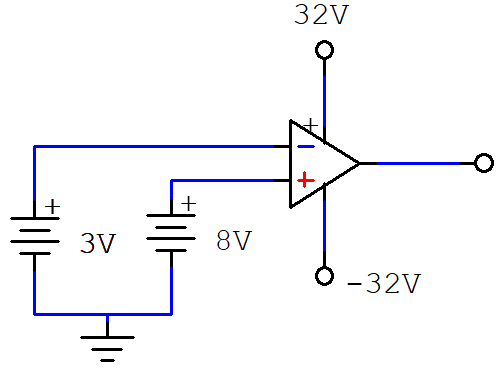
\includegraphics[width=\textwidth]{operasjonsforsterker/figurer/basic1.png}
			\caption{Kobling 1}
			\label{fig:basicOpamp1}
		\end{minipage}\hfill
		\begin{minipage}{0.45\textwidth}
			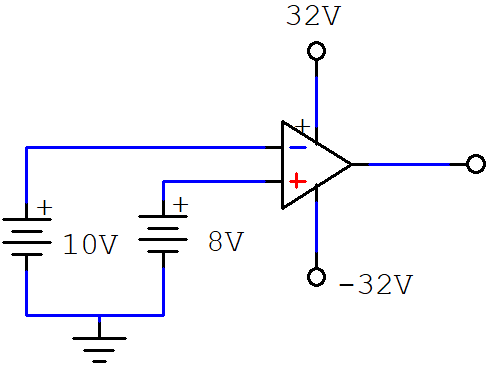
\includegraphics[width=\textwidth]{operasjonsforsterker/figurer/basic2.png}
			\caption{Kobling 2}
			\label{fig:basicOpamp2}
		\end{minipage}\par
		\vskip\floatsep% normal separation between figures
		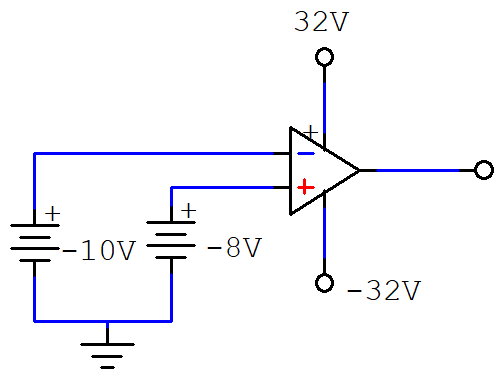
\includegraphics[width=0.45\textwidth]{operasjonsforsterker/figurer/basic3.png}
		\caption{Kobling 3}
		\label{fig:basicOpamp3}
	\end{figure}

\end{question}

\vspace{0.5cm} % Add space after the solution

\begin{solution}[name=Løsningsforslag oppgave]
Kobling 1: $U_{ut}=32[V]$

Potensialet på den ikke-inverterende inngangen er høyere enn potensialet på den inverterende. Utgangen vil derfor gå til maksimum positiv spenning bare begrenset av driftspenningen til kretsen.

Kobling 2: $U_{ut}=-32[V]$

Potensialet på den inverterende inngangen er høyere enn potensialet på den ikke-inverterende. Utgangen vil derfor gå til maksimum negativ spenning bare begrenset av driftspenningen til kretsen.

Kobling 3: $U_{ut}=32[V]$

Potensialet på den inverterende inngangen er høyere enn potensialet på den ikke-inverterende ved at spenningen på den ikke-inverterende er mindre negativt enn potensialet på den inverterende. Utgangen vil derfor gå til maksimum positiv spenning bare begrenset av driftspenningen til kretsen.

\end{solution}
\vspace{0.5cm} % Add space after the solution

%--------------------------- INVERTERNENDE KOBLING --------------------------------
\begin{question}[name=Oppgave, topic=operasjonsforsterker]
En operasjonsforsterkerkrets er koblet som inverterende forsterker. Kretsens forsterkning $F_U = -200$ med en inngangsresistans / serieresistans angitt til $R_1=10[k\Omega]$.

	\begin{enumerate}[label=\roman*)]
		\item Beregn motstandsverdien for $R_2$.
		\item Hva er spenningen man måler man på utgangen av koblingen, dersom inngangspenningen er $1[V_{DC}]$
	\end{enumerate}


\end{question}

\vspace{0.5cm} % Add space after the solution

\begin{solution}[name=Løsningsforslag oppgave]

		\begin{enumerate}[label=\roman*)]
		\item
\[F_U =- \frac{R_K}{R_1} \rightarrow -200= \frac{R_K}{10 \cdot 10^3} \rightarrow -200 \cdot 10 \cdot 10^3 = -R_K \rightarrow R_K = 200 \cdot 10 \cdot 10^3 = 2[M\Omega]\]

		\item
\[U_{ut}=-\frac{R_K}{R_{inn}} \cdot U_{inn} = -\frac{2\cdot 10^6}{10 \cdot 10^3} \cdot 1 = -200[V]\]

Operasjonsforsterkerens utgangspenning blir begrense av $\pm V_{CC}$.
	\end{enumerate}

\end{solution}
\vspace{0.5cm} % Add space after the solution

\begin{question}[name=Oppgave, topic=operasjonsforsterker]
		\begin{enumerate}[label=\roman*)]
			\item Kretsen som vist i Figur \ref{fig:invKobling} er koblet slik at forsterkningen $F_U = 2$. Kretsen blir påtrykt et signal som vist i Figur \ref{fig:invPlot}. Tegn utgangsignalet sammen med inngangsignalet for kretsen.

			\item Si noe om hvordan forholdet mellom $R_1$ og $R_2$ må være for at kretsen skal ha $F_U = 2$. Foreslå motstandsverdier for $R_1$ og $R_2$.
		\end{enumerate}
	\begin{figure}[H]
	\begin{minipage}[c]{0.45\linewidth}
		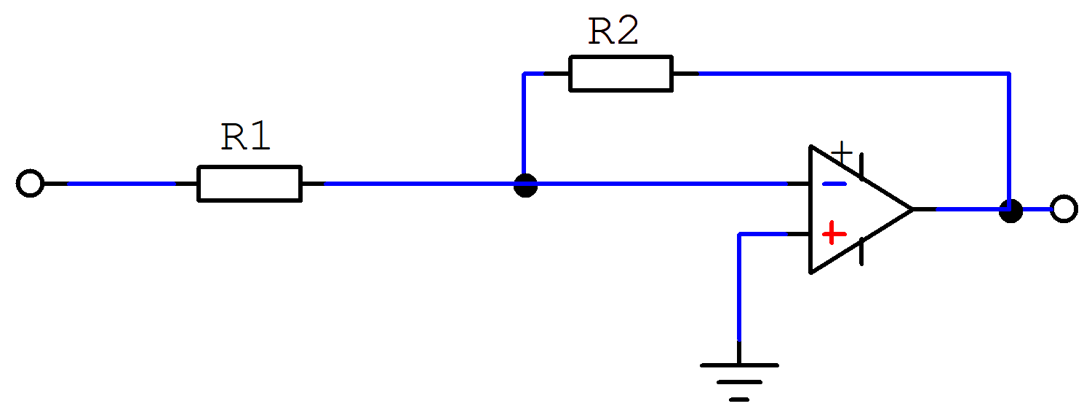
\includegraphics[width=\linewidth]{operasjonsforsterker/figurer/invBasic.png}
		\caption{Krets med operasjonforsterker}
		\label{fig:invKobling}
	\end{minipage}
	\hfill
	\begin{minipage}[c]{0.45\linewidth}
		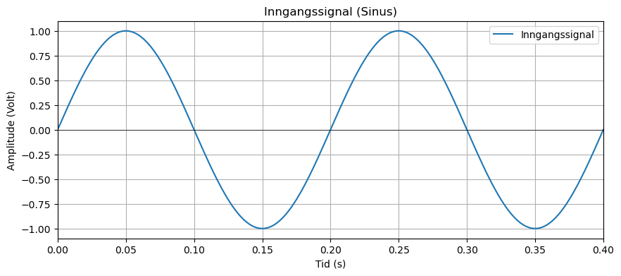
\includegraphics[width=\linewidth]{operasjonsforsterker/plot/InvPlot.png}
		\caption{Inngangsignal til krets}
		\label{fig:invPlot}
	\end{minipage}
\end{figure}

\end{question}

\vspace{0.5cm} % Add space after the solution

\begin{solution}[name=Løsningsforslag oppgave]
		\begin{enumerate}[label=\roman*)]
	\item
		\begin{figure}[H]
		\centering
		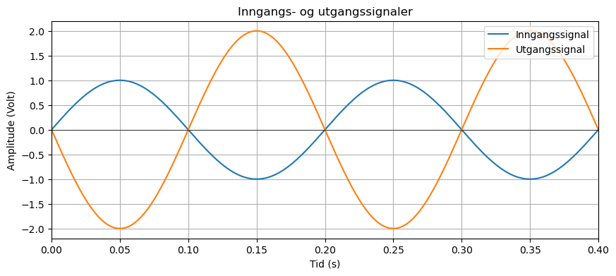
\includegraphics[width=0.7\textwidth]{operasjonsforsterker/plot/InvPlotSOL.png}
		\caption{Inngang og utgangsignal for en inverterende kobling}
		\label{fig:invPlotSOL}
	\end{figure}
	\item Den generelle spenningsforsterkningen for en inverterende kobling kan beskrives ved formelen som vist i Formel \ref{eqn:opAmpForsterk}.

	\begin{equation}
		\label{eqn:opAmpForsterk}
		F_U = -\frac{R_K}{R_{inn}}
	\end{equation}

Dersom man ønsker er forsterkning $F_U=-1$ vil det si at $R_K$ og $R_{inn}$ må ha samme verdi slik at når de deles på hverandre blir resultatet 1. Dersom man ønsker en dobling av forsterkningen må tallet i teller være dobbelt så stort som i nevner for at resultatet skal bli 2. Et eksempel:

\[F_U=-\frac{2}{1}=2\]

Så ved en teoretisk betraktning kan man derfor si at forholdet mellom motstandene sier noe om forsterkningen, og ikke verdien på motstandene. Derfor kan alternative verdier være $R_K=2 [\Omega]$ og $R_{inn}=1[\Omega]$, eller $R_K=2 [M\Omega]$ og $R_{inn}=1[M\Omega]$

\end{enumerate}
\end{solution}
\vspace{0.5cm} % Add space after the solution


\begin{question}[name=Oppgave, topic=operasjonsforsterker]
Finn verdien for $R_2$ i for kretsen vist i Figur \ref{fig:invCircuit1} slik at $F_U=100$.
\begin{figure}[H]
	\centering
	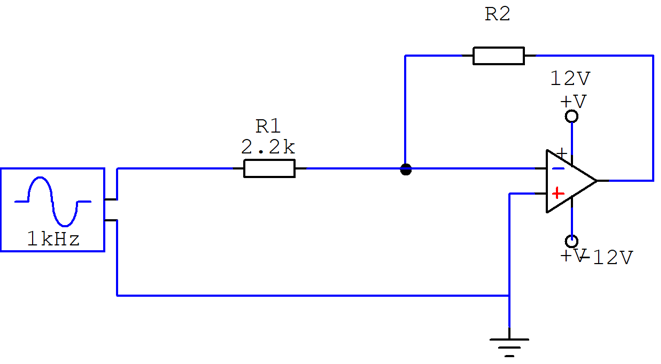
\includegraphics[width=0.7\textwidth]{operasjonsforsterker/figurer/invBasicCir.png}
	\caption{Operasjonsforsterkerkrets}
	\label{fig:invCircuit1}
\end{figure}

\end{question}

\vspace{0.5cm} % Add space after the solution

\begin{solution}[name=Løsningsforslag oppgave]

\[F_U = -\frac{R_2}{R_1} \rightarrow -100 = -\frac{R_2}{2,2 \cdot 10^{3}} \rightarrow (-100) \cdot 2,2 \cdot 10^3 = -R_2 \cdot 1 \rightarrow R_2 = 220 [k\Omega]\]

\end{solution}
\vspace{0.5cm} % Add space after the solution


%--------------------------- IKKE INVERTERNENDE KOBLING --------------------------------


\begin{question}[name=Oppgave, topic=operasjonsforsterker]

Kretsen som vist i Figur \ref{fig:NONinvKobling} er koblet slik at forsterkningen $F_U = 2$. Kretsen blir påtrykt et signal som vist i Figur \ref{fig:NONinvPlot}. Tegn utgangsignalet sammen med inngangsignalet for kretsen.

	\begin{figure}[H]
		\begin{minipage}[c]{0.45\linewidth}
			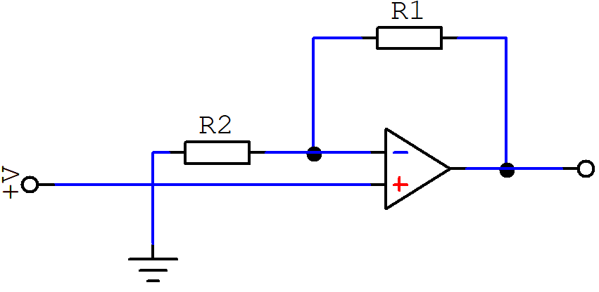
\includegraphics[width=\linewidth]{operasjonsforsterker/figurer/NONinvBasic.png}
			\caption{Krets med operasjonforsterker}
			\label{fig:NONinvKobling}
		\end{minipage}
		\hfill
		\begin{minipage}[c]{0.45\linewidth}
			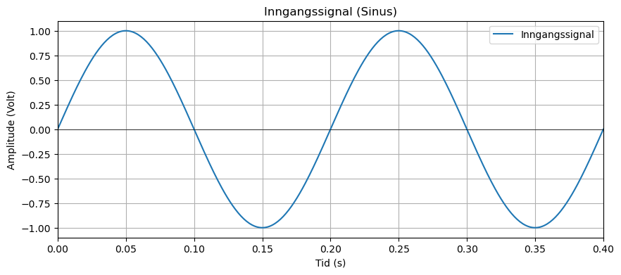
\includegraphics[width=\linewidth]{operasjonsforsterker/plot/NONInvPlot.png}
			\caption{Inngangsignal til krets}
			\label{fig:NONinvPlot}
		\end{minipage}
	\end{figure}

\end{question}

\vspace{0.5cm} % Add space after the solution

\begin{solution}[name=Løsningsforslag oppgave]


\begin{figure}[H]
	\centering
	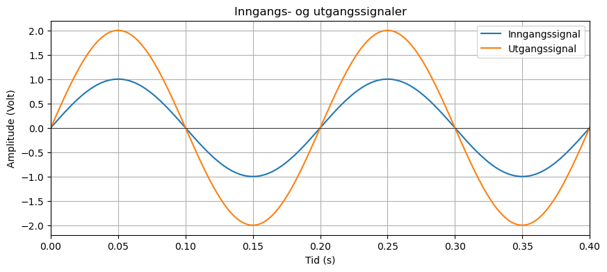
\includegraphics[width=0.7\textwidth]{operasjonsforsterker/plot/NONInvPlotSOL.png}
	\caption{Inn og utgangsignal for kretsen}
	\label{fig:NONinvPlotSol}
\end{figure}

\end{solution}
\vspace{0.5cm} % Add space after the solution

\begin{question}[name=Oppgave, topic=operasjonsforsterker]
Finn verdien for $R_2$ slik at forsterkningen blir 100.
	\begin{figure}[H]
	\centering
	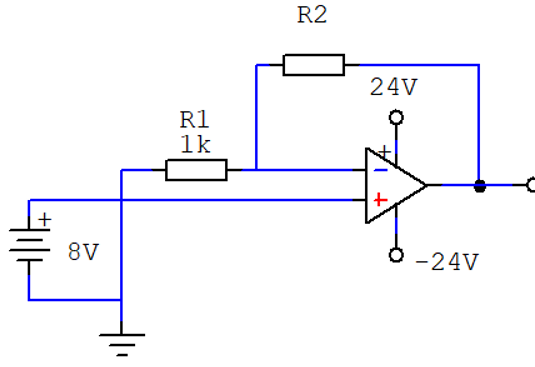
\includegraphics[width=0.6\textwidth]{operasjonsforsterker/figurer/NONinvBasic2.png}
	\caption{Operasjonsforsterkerkrets}
	\label{fig:NONinvKrets2}
\end{figure}

\end{question}

\vspace{0.5cm} % Add space after the solution

\begin{solution}[name=Løsningsforslag oppgave]
\[F_U=1+\frac{R_2}{R_1} \rightarrow 100=1+\frac{R_2}{1 \cdot 10^3} \rightarrow 100-1=\frac{R_2}{1 \cdot 10^3} \rightarrow R_2=99 \cdot 10^3=99[k\Omega] \]

\end{solution}
\vspace{0.5cm} % Add space after the solution

\begin{question}[name=Oppgave, topic=operasjonsforsterker]
Finn verdien for $U_{ut}$ i Figur \ref{fig:NONinvKrets3}.
	\begin{figure}[H]
		\centering
		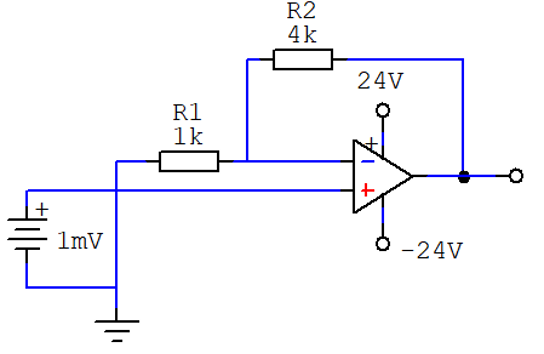
\includegraphics[width=0.6\textwidth]{operasjonsforsterker/figurer/NONinvBasic3.png}
		\caption{Operasjonsforsterkerkrets}
		\label{fig:NONinvKrets3}
	\end{figure}

\end{question}

\vspace{0.5cm} % Add space after the solution

\begin{solution}[name=Løsningsforslag oppgave]
\[U_{ut}= \left(1+\frac{R_2}{R_1}\right) \cdot U_{inn} = \left(1+\frac{4\cdot 10^3}{1 \cdot 10^3}  \right) \cdot 4 = \left(1+4 \right) \cdot 4 = 20[V]\]
\end{solution}
\vspace{0.5cm} % Add space after the solution

\begin{question}[name=Oppgave, topic=operasjonsforsterker]
Finn spenningsforsterkningen og utgangspenningen for kretsen vist i Figur \ref{fig:NONinvKrets4}.
	\begin{figure}[H]
		\centering
		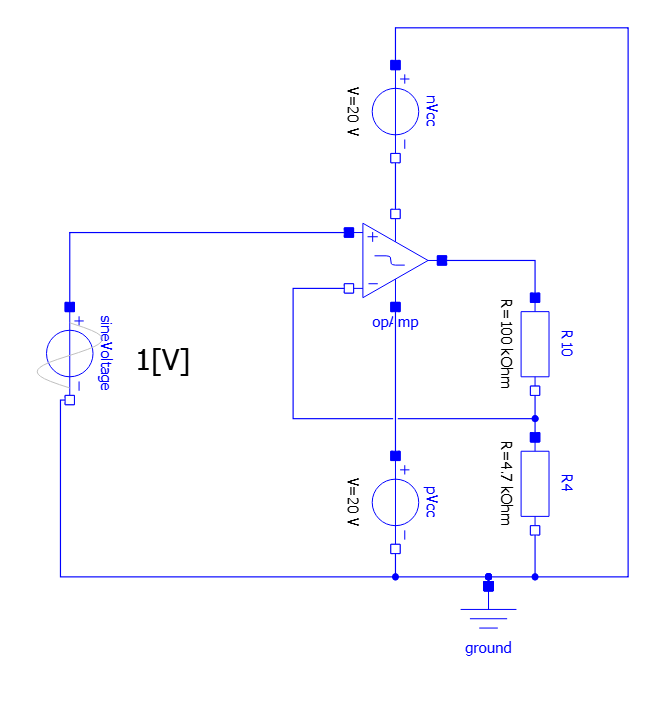
\includegraphics[width=0.6\textwidth]{operasjonsforsterker/figurer/NONinvBasic4.png}
		\caption{Operasjonsforsterkerkrets}
		\label{fig:NONinvKrets4}
	\end{figure}

\end{question}

\vspace{0.5cm} % Add space after the solution

\begin{solution}[name=Løsningsforslag oppgave]
\[F_U= 1+\frac{R_{10}}{R_4} = 1+ \frac{100\cdot10^3}{4,7\cdot10^3} = 22,3 \]

Med inngangsignal $U_{inn}=1[V]$ som merket i kretsen kan man beregne utgangspenningen.

\[U_{ut}=U_{inn} \cdot F_U= 1 \cdot 22,3 = 22,3[V]\]

Siden operasjonsforsterkeren er forsynt med $\pm 20[V]$ vil maksimal spenning på utgangen bli $20[V]$ som vist i simulering av kretsen i Figur \ref{fig:NONinvKrets4PLOT} hvor signalet holdes konstant ved $20[V]$ før utgangen faller under eller over $20[V]$ igjen.
	\begin{figure}[H]
	\centering
	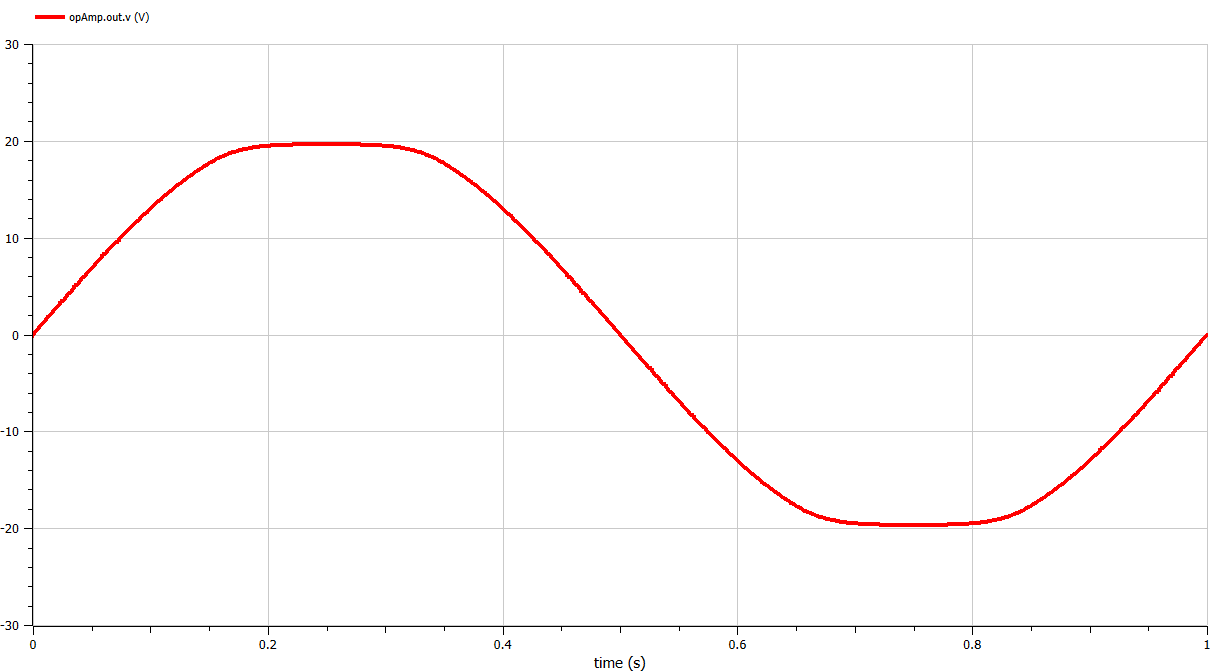
\includegraphics[width=0.6\textwidth]{operasjonsforsterker/plot/NONinvBasic4PLOT.png}
	\caption{Operasjonsforsterkerkrets - Plot}
	\label{fig:NONinvKrets4PLOT}
\end{figure}



\end{solution}
\vspace{0.5cm} % Add space after the solution




%--------------------------- SUMMERENDE KOBLING --------------------------------
\begin{question}[name=Oppgave, topic=operasjonsforsterker]
	Finn hvilken spenning måler man på utgangen av kretsen vist i \ref{fig:sumCircuit2}.

	\begin{figure}[H]
		\centering
		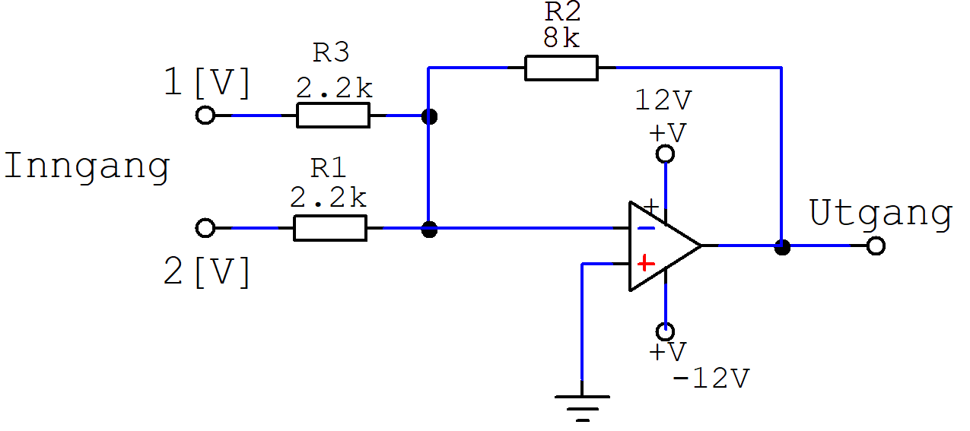
\includegraphics[width=0.8\textwidth]{operasjonsforsterker/figurer/SumKrets1.png}
		\caption{Operasjonsforsterkerkrets}
		\label{fig:sumCircuit2}
	\end{figure}

\end{question}

\vspace{0.5cm} % Add space after the solution

\begin{solution}[name=Løsningsforslag oppgave]
Løsningsalternativ 1:

Beregner de individuelle spenningsforsterkningene.
\[F_1=-\frac{R_2}{R_3}=\frac{8\cdot10^3}{2,2\cdot10^3} \approx -3,636\]
\[F_2=-\frac{R_2}{R_1}=\frac{8\cdot10^3}{2,2\cdot10^3} \approx -3,636\]

Beregner så utgangspenningen.
\[U_{ut}=F_1 \cdot U_{inn1}+F_2 \cdot U_{inn2}=3,636\cdot1+3,636\cdot2\approx 10,9[V]\]

Løsningsalternativ 2:
\[U_{ut}=- \left (\frac{U_{inn1}}{R_3}+\frac{U_{inn2}}{R_1} \right) = -\left (\frac{1}{2,2\cdot10^3}+\frac{2}{2,2\cdot10^3} \right) \cdot 8 \cdot10^3 = \frac{120}{11} \approx10,9[V]\]

\end{solution}
\vspace{0.5cm} % Add space after the solution

\begin{question}[name=Oppgave, topic=operasjonsforsterker]
Finn hvilken spenning måler man på utgangen av kretsen vist i \ref{fig:sumCircuit1}.

	\begin{figure}[H]
		\centering
		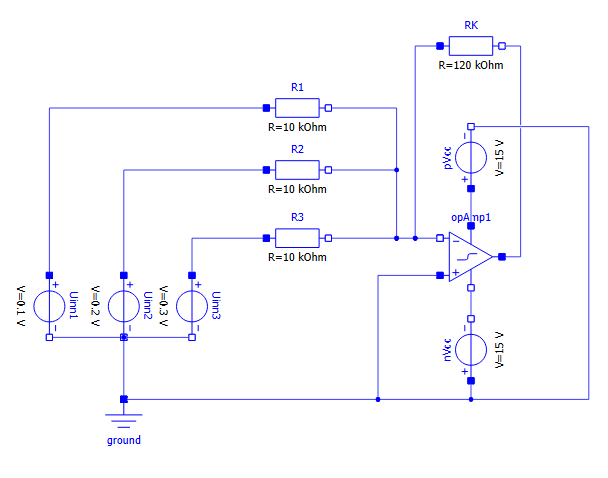
\includegraphics[width=0.8\textwidth]{operasjonsforsterker/figurer/SumKrets.png}
		\caption{Operasjonsforsterkerkrets}
		\label{fig:sumCircuit1}
	\end{figure}

\end{question}

\vspace{0.5cm} % Add space after the solution

\begin{solution}[name=Løsningsforslag oppgave]

\[U_{ut}=-\left(\frac{U_{inn1}}{R_1}+\frac{U_{inn2}}{R_2}+\frac{U_{inn3}}{R_3}\right)\cdot R_K = -\left(\frac{0,1}{10 \cdot10^3}+\frac{0,2}{10 \cdot10^3}+\frac{0,3}{10 \cdot10^3}\right)\cdot 120 \cdot 10^3 = -7,2 [V]\]

\end{solution}

\vspace{0.5cm} % Add space after the solution
\subsection{Løsningsforslag}
\printsolutions[section]




\newpage


\chapter{Måleteknikk}
\section{Måleusikkerhet}
\subsection{Absolutt Usikkerhet}

Absolutt usikkerhet refererer til den faktiske mengden usikkerhet i en måling, uttrykt i samme enhet som selve målingen. For eksempel, hvis du måler lengden av et bord til 2,00 meter med en usikkerhet på ±0,01 meter, er den absolutte usikkerheten 0,01 meter. Denne typen usikkerhet brukes ofte når man ønsker å vite den eksakte mengden usikkerhet i en måling.

\subsection{Relativ Usikkerhet}

Relativ usikkerhet er forholdet mellom den absolutte usikkerheten og selve målingen, og den uttrykkes ofte som en prosentandel. Formelen for relativ usikkerhet er:

\begin{equation}
	\label{eqn:relUsikkerhet}
		 	Relativ\ usikkerhet = \frac{Absolutt\ usikkerhet}{M \text{å}lt verdi} \cdot 100 \%
\end{equation}



For eksempel, hvis du har en måling på 2,00 meter med en absolutt usikkerhet på ±0,01 meter, er den relative usikkerheten $\frac{0,01}{2,00} \cdot 100 \% = 0,5\%$. Relativ usikkerhet brukes ofte for å sammenligne usikkerheten i forskjellige målinger eller for å vurdere nøyaktigheten av en måling i forhold til størrelsen på målingen.


\section{Oppgaver}
\begin{comment}

	\begin{question}[name=Oppgave, topic=måleusikkerhet]

		\begin{enumerate}[label=\roman*)]

		\end{enumerate}
	\end{question}

	\vspace{0.5cm} % Add space after the solution

	\begin{solution}[name=Løsningsforslag oppgave]

		\begin{figure}[H]
			\centering
			\includegraphics[width=0.7\textwidth]{}
			\caption{}
			\label{fig:}
		\end{figure}
	\end{solution}

	\vspace{0.5cm} % Add space after the solution
\end{comment}



\begin{question}[name=Oppgave, topic=måleusikkerhet]
Lengden på et bord er målt til å være 2 meter. Nøyaktigheten på målinger er $0,2\%$ med en repeterbarhet på $0,05 \%$. Utfør følgende:

	\begin{enumerate}[label=\roman*)]
		\item Beregn total usikkerhet
		\item Beregn absolutt usikkerhet
		\item Beskriv målingen med korrekt usikkerhet
	\end{enumerate}


\end{question}

\vspace{0.5cm} % Add space after the solution

\begin{solution}[name=Løsningsforslag oppgave]
	\begin{enumerate}[label=\roman*)]
	\item Total usikkerhet
\[Total\ usikkerhet = Nøyaktighet + Repeterbarhet = 0,2 \% + 0,05 \% = 0,25 \% \]
	\item Absolutt usikkerhet
\[Absolutt\ usikkerhet = M\text{å}lt verdi \cdot \frac{Total\ usikkerhet}{100}=2 \cdot \frac{0,25}{100}=0,005[m]\]
	\item Beskriv målingen med korrekt usikkerhet
\[(2 \pm 0,005) [m]\]
	\end{enumerate}
\end{solution}

\vspace{0.5cm} % Add space after the solution



\begin{question}[name=Oppgave, topic=måleusikkerhet]
Temperaturen i en ovn måles til $200 [^\circ C]$. Nøyaktigheten i målingen er $0,1 \% $  med en repeterbarhet på $0,002 \%$. Utfør følgende:


	\begin{enumerate}[label=\roman*)]
		\item Total usikkerhet
		\item Absolutt usikkerhet
	\end{enumerate}


\end{question}

\vspace{0.5cm} % Add space after the solution

\begin{solution}[name=Løsningsforslag oppgave]
	\begin{enumerate}[label=\roman*)]
		\item Total usikkerhet
\[Total\ usikkerhet = Nøyaktighet + Repeterbarhet = 0,1 \% + 0,02 \% = 0,12 \% \]
		\item Absolutt usikkerhet
\[Absolutt\ usikkerhet = M\text{å}lt\ verdi \cdot \frac{Usikkerhet}{100}=200 \cdot \frac{0,12}{100}=0,24 [^\circ C]\]
	\end{enumerate}
\end{solution}

\vspace{0.5cm} % Add space after the solution




\begin{question}[name=Oppgave, topic=måleusikkerhet]
For å øke nøyaktigheten på en måling av væskenivå i en tank blir det utført uavhengige målinger etter hverandre. Målingene gir følgende resultater: $49,8[l]$, $50,2[l]$, $50,0[l]$. Nøyaktigheten i målingene er $0,3 \%$ med en repeterbarhet på $0,01 \%$. Utfør følgende:

	\begin{enumerate}[label=\roman*)]
		\item Beregn total usikkerhet
		\item Beregn absolutt usikkerhet
		\item Beskriv målingen med korrekt usikkerhet
	\end{enumerate}


\end{question}

\vspace{0.5cm} % Add space after the solution

\begin{solution}[name=Løsningsforslag oppgave]
	\begin{enumerate}[label=\roman*)]
		\item Finner gjennomsnittsverdien for målingene
\[Gjennomsnitt= \frac{Summen\ av\ alle\ m\text{å}linger}{Antall\ m\text{å}linger}= \frac{49,8+50,2+50,0}{3}=50,0[l]\]

		\item Absolutt usikkerhet

		\item Beskriv målingen med korrekt usikkerhet

	\end{enumerate}
\end{solution}




\begin{question}[name=Oppgave, topic=måleusikkerhet]
En brygger måler volumet av øl ved hjelp av en målesylinder. Målesylinderen har en nøyaktighet på $\pm 0,3 \%$ og en repeterbarhet på $0,01 \%$. Det er utført 10 målinger på en produksjonsenhet med øl, som ga følgende resultat: $50,050[l]$, $49,813[l]$, $50,030[l]$, $50,089[l]$, $49,838[l]$, $50,038[l]$, $49,928[l]$, $50,131[l]$, $50,141[l]$, $49,893[l]$. Utfør følgende:

\begin{enumerate}[label=\roman*)]
	\item Beregn total usikkerhet
	\item Beregn absolutt usikkerhet
	\item Beskriv målingen med korrekt usikkerhet
\end{enumerate}

\end{question}

\vspace{0.5cm} % Add space after the solution

\begin{solution}[name=Løsningsforslag oppgave]
	\begin{enumerate}[label=\roman*)]
	\item Total usikkerhet

		Beregner gjennomsnittet
		\[\mu = 50,050 + 49,813 + 50,030 + 50,089 + 49,838 + 50,038 + 49,928 + 50,131 + 50,141 + 49,893 = 49,995[l]\]

		Total usikkerhet
		\[Total\ usikkerhet = Nøyaktighet + Repeterbarhet = 0,3 + 0,01 = 0,31 \%\]
	\item Absolutt usikkerhet
		\[Absolutt\ usikkerhet = \mu \cdot \frac{Total\ usikkerhet}{100}= 49,995 \cdot \frac{0,31}{100}=0,155 [l]\]

	\item Beskriv målingen med korrekt usikkerhet
		\[(49,995 \pm 0,155) [l]\]

	\end{enumerate}
\end{solution}



\begin{question}[name=Oppgave, topic=måleusikkerhet]
Multimetere vist i Figur \ref{fig:zoyiMul} ble benyttet til å måle en DC-spenning. Instrumentet ga verdien $46,5 [V]$.
	\begin{enumerate}[label=\roman*)]
		\item Med utgangspunkt i data presentert i Figur \ref{fig:zoyiDat} beskriv hvordan det påvirker en måling dersom man bruker et høyere måleområde enn nødvendig
		\item Beregn usikkerhet og vis måleresultatet med usikkerheten, basert på databladet til instrumentet vist i Figur \ref{fig:zoyiDat}.
	\end{enumerate}
Beregn usikkerhet og vis måleresultatet med usikkerheten basert på databladet til instrumentet vist i Figur \ref{fig:zoyiDat}.

	\begin{figure}[H]
		\begin{minipage}[c]{0.45\linewidth}
			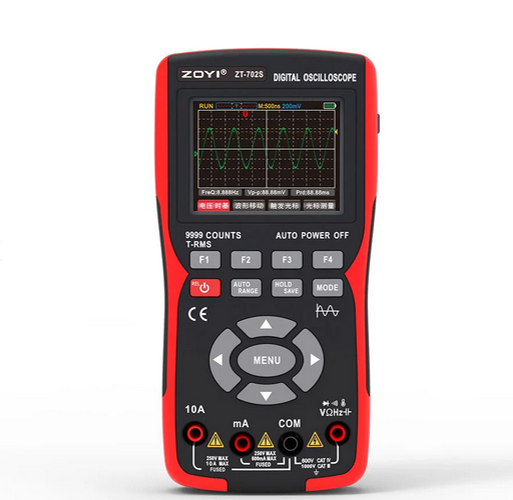
\includegraphics[width=\linewidth]{måleteknikk/figurer/zoyiMultimeter.png}
			\caption{Bilde av måleinstrument}
			\label{fig:zoyiMul}
		\end{minipage}
		\hfill
		\begin{minipage}[c]{0.45\linewidth}
			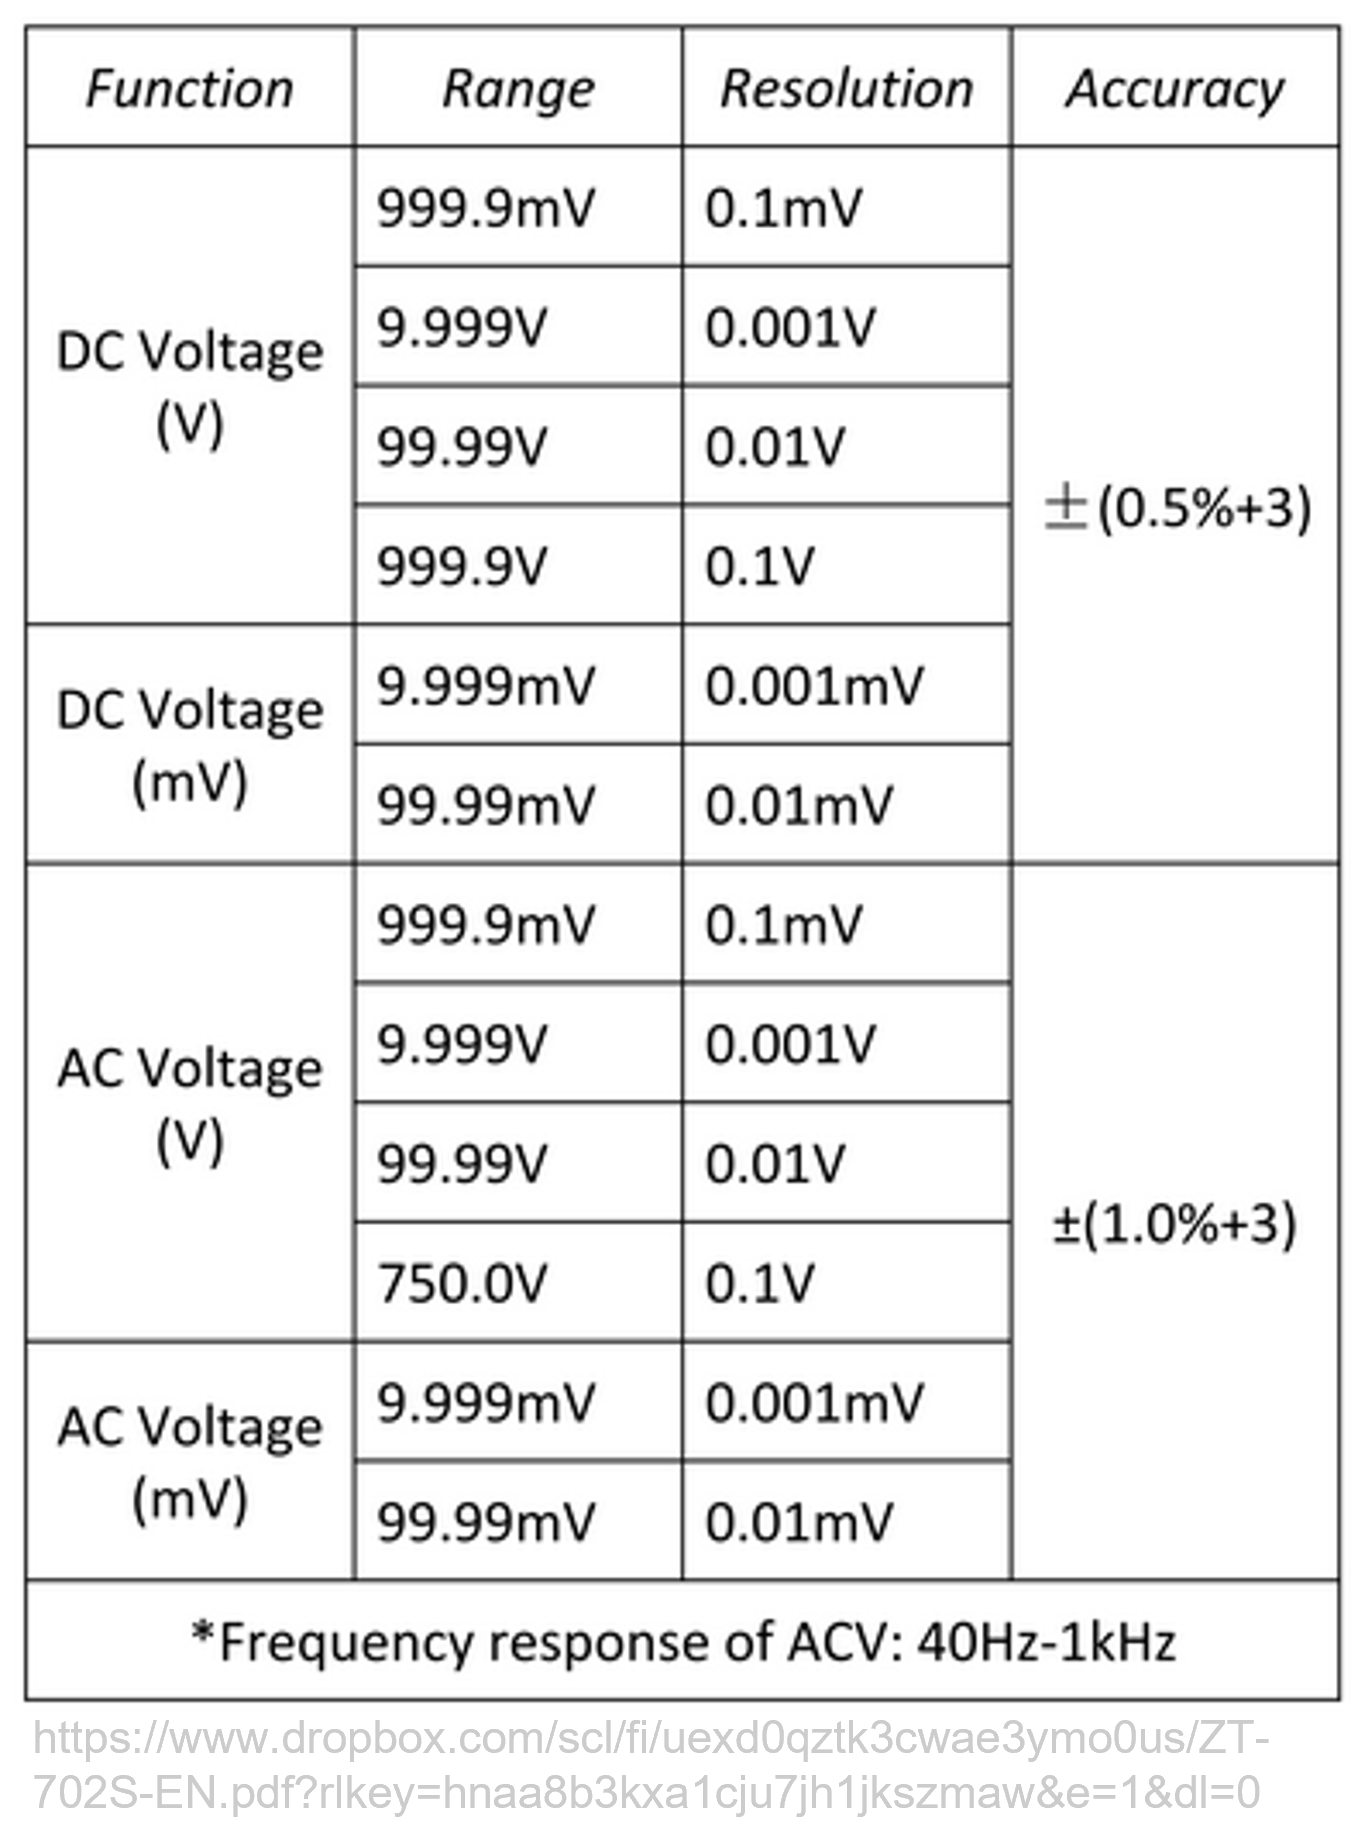
\includegraphics[width=\linewidth]{måleteknikk/figurer/zoyiData.png}
			\caption{Utdrag fra datablad}
			\label{fig:zoyiDat}
		\end{minipage}
	\end{figure}

\end{question}
\vspace{0.5cm} % Add space after the solution

\begin{solution}[name=Løsningsforslag oppgave]
	\begin{enumerate}[label=\roman*)]
	\item Måleinstrumentet vil få en redusert nøyaktighet siden oppløsningen (Resolution) vil reduseres. Dersom man måler $8 [V]$ med måleområde $999,9 [V]$ vil den konstante usikkerheten være på $0,3 [V]$. Hvis man i stede bruker det nærmeste området for målingen som er $9,999 [V]$ vil den konstante usikkerheten være redusert til $0,003 [V]$

	\item Leser av den prosentvise relative usikkerheten fra tabellen til å være $0,5 \%$. Beregner så den absolutte usikkerheten.
	\[Usikkerhet = M\text{å}ling \cdot \frac{Relativ\ usikkerhet}{100}=46,5 \cdot \frac{0,5}{100}=0,235[V]\]

	Leser av den konstante absolutte usikkerheten fra tabellen til å være $3$, og oppløsningen til å være $0,01[V]$.
	\[Usikkerhet_{konst}= Oppløsning \cdot konstant_{usikkerhet} = 3 \cdot 0,01 = 0,03 [V]\]

	Beregner den totale måleusikkerheten
	\[Total\ usikkerhet = Usikkerhet + Usikkerhet_{konst}=0,235+0,03=265 [mV]\]

	Måleresultatet kan beskrive ved:
	\[(46,5 \pm 0,265) [V]\]


\end{enumerate}


\end{solution}
\section{Løsningsforslag}
\printsolutions[chapter]


\newpage
\chapter{Referanser}
\printbibliography[heading=none]

%\printbibheading[title={Referanser}]
%\printbibliography[keyword=datablad, heading=subbibliography, title={Datablad}]
%\printbibliography[type=online, heading=subbibliography, title={Bøker}]
\appendix


\chapter[LED Datasheet]{LED Datasheet}
\label{paper-a}

\emph{Datablad fra en standard LED \cite{LEDdatasheet}.}
	
	\bigskip

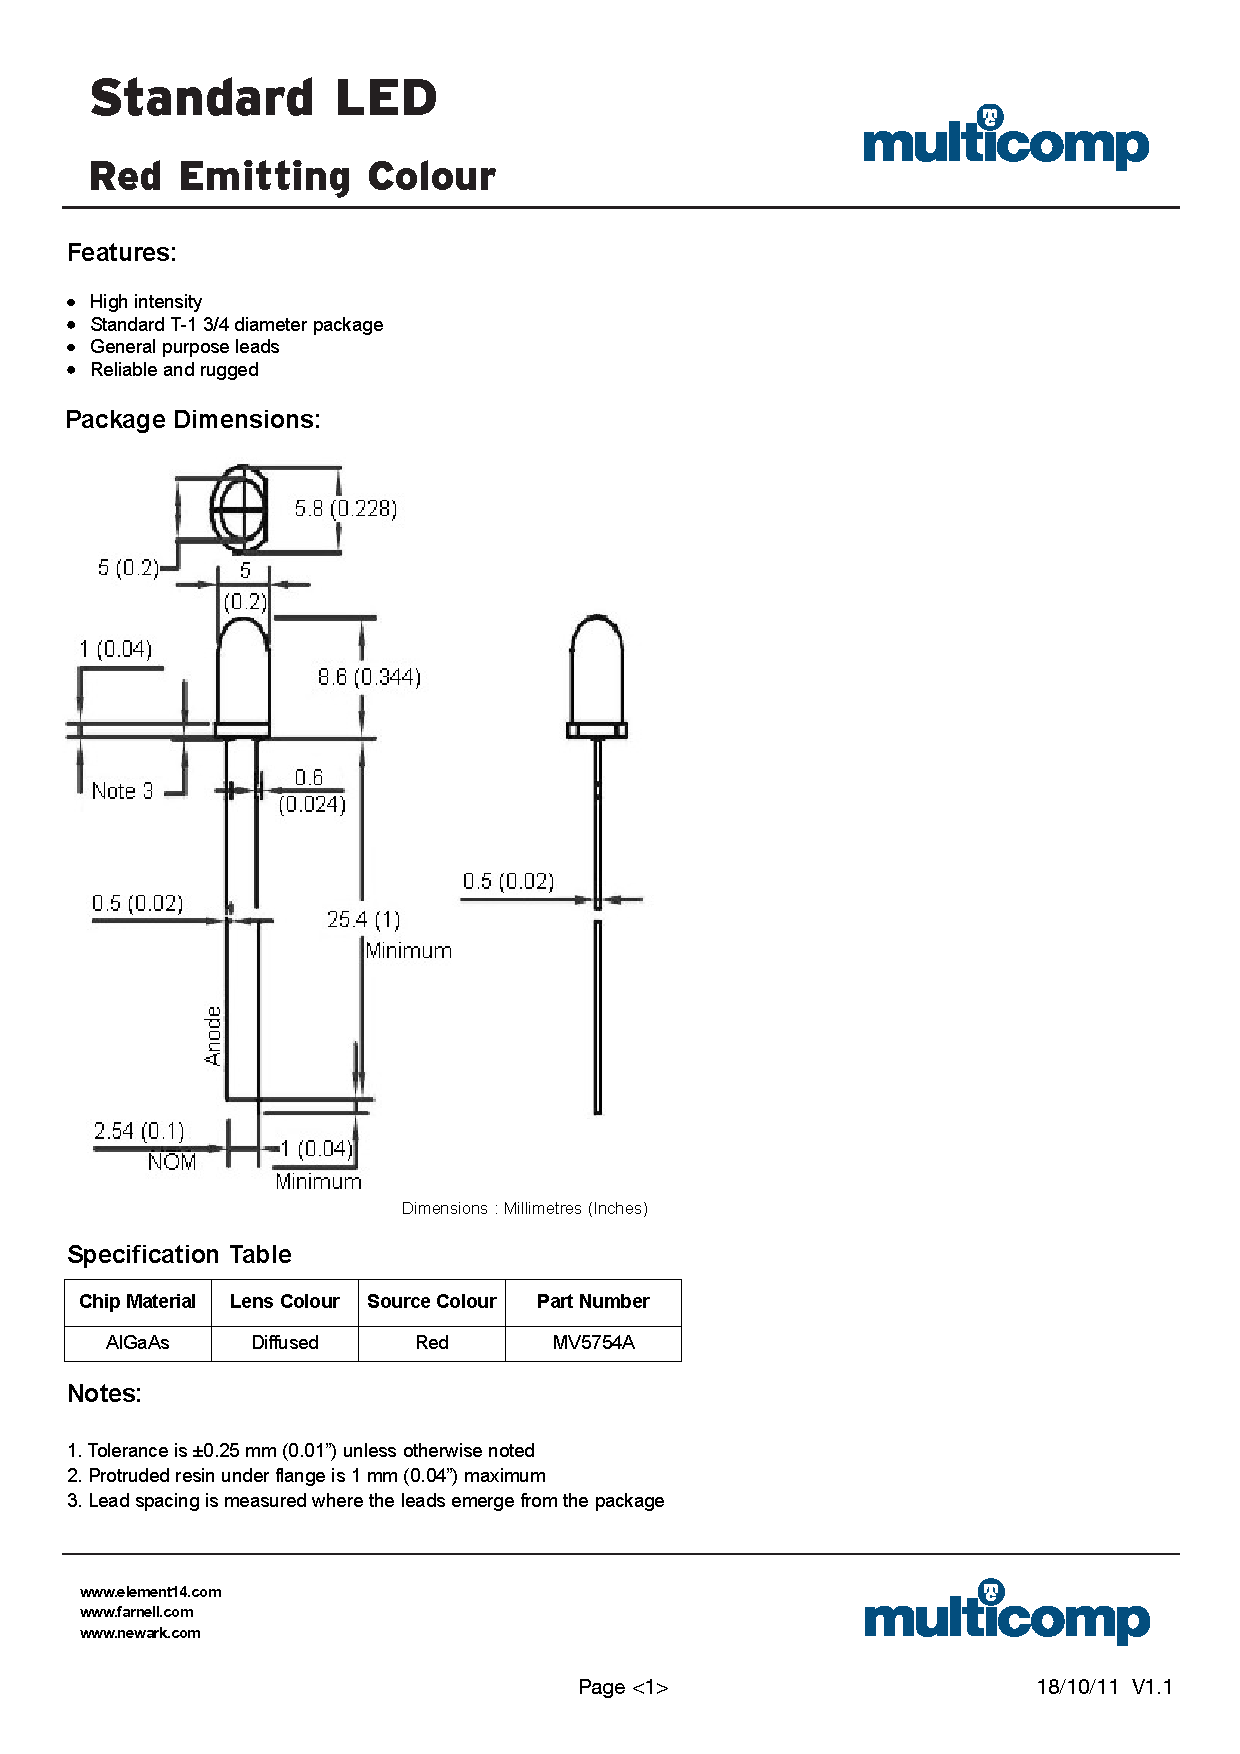
\includepdf[pages=-]{backmatter/pdfVedlegg/1LED_datasheet1498852.pdf}




\end{document}
